\documentclass[border=3pt]{standalone}
\usepackage{amsmath,amssymb,xcolor,fontspec,tikz}
\usetikzlibrary{arrows.meta,angles,quotes,positioning}
\setmainfont{NimbusRoman-Regular.otf}[Path=/usr/share/fonts/opentype/urw-base35/,BoldFont=NimbusRoman-Bold.otf,ItalicFont=NimbusRoman-Italic.otf,BoldItalicFont=NimbusRoman-BoldItalic.otf]
\definecolor{fg}{HTML}{FFFFFF}\definecolor{bg}{HTML}{000000}
\definecolor{yel}{HTML}{FFD45C}\definecolor{cya}{HTML}{70DCF5}

\begin{document}
\pagecolor{bg}\color{fg}
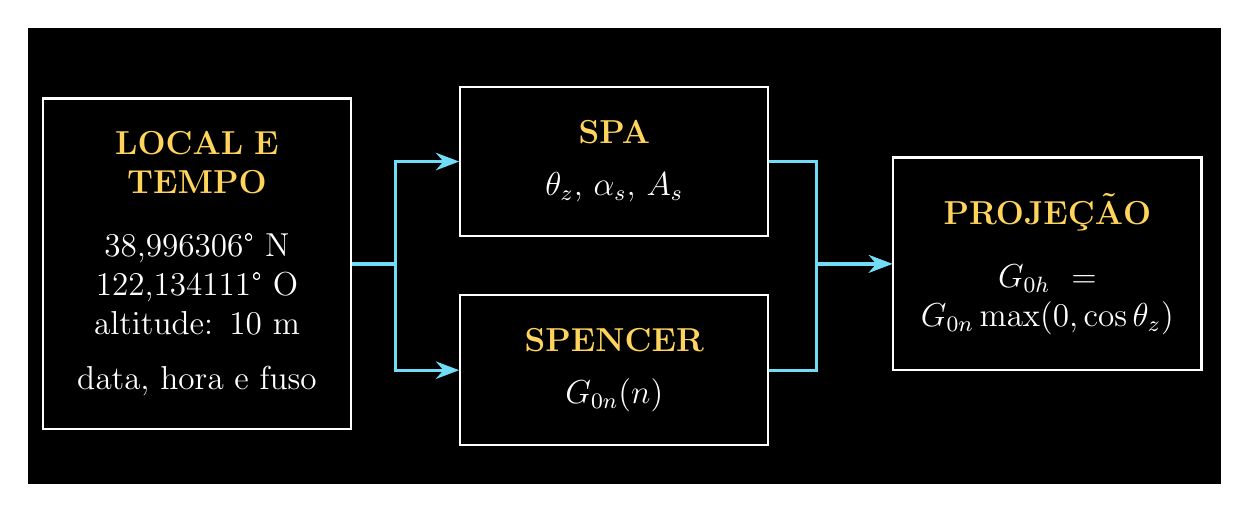
\begin{tikzpicture}[x=1cm,y=1cm,>=Stealth,font=\large,
 box/.style={draw=fg,thick,text=fg,align=center,minimum height=1.9cm,text width=3.35cm,inner sep=8pt}]
\path[fill=bg](-.35,-1.45)rectangle(14.8,4.35);
\node[box,minimum height=4.2cm] (in) at(1.8,1.35){\textcolor{yel}{\textbf{LOCAL E TEMPO}}\\[9pt]38,996306° N\\122,134111° O\\altitude: 10 m\\[6pt]data, hora e fuso};
\node[box] (spa) at(7.1,2.65){\textcolor{yel}{\textbf{SPA}}\\[5pt]$\theta_z$, $\alpha_s$, $A_s$};
\node[box] (sp) at(7.1,0){\textcolor{yel}{\textbf{SPENCER}}\\[5pt]$G_{0n}(n)$};
\node[box,minimum height=2.7cm] (out) at(12.6,1.35){\textcolor{yel}{\textbf{PROJEÇÃO}}\\[9pt]$G_{0h}=$\\$G_{0n}\max(0,\cos\theta_z)$};
\draw[cya,->,very thick](in.east)--++(.55,0)|-(spa.west);
\draw[cya,->,very thick](in.east)--++(.55,0)|-(sp.west);
\draw[cya,->,very thick](spa.east)--++(.6,0)|-(out.west);
\draw[cya,->,very thick](sp.east)--++(.6,0)|-(out.west);
\end{tikzpicture}
\end{document}
